\section{Theory}
\label{sec:theory}

The following section explains the theoretical principles of a diode laser.

\subsection{Historical Background}
\label{sec:Historical Background}

Before semiconductor lasers were invented, physicists used tunable 'dye' lasers.
This worked by the use of a chemical dye as the active medium, i.e the material which produces the laser emission.
A fixed-frequency 'pump'-laser is used to create a population inversion. Each individual dye will lase over a limited wavelenght range.
This means with different dyes it is possible to generate a tunable lasers at basically all near-infrared wavelenghts.
Dye Lasers have some disadvantages. They are very large, with high costs of purchase and operation.

The situation has changed due to the development of the diode laser. These lasers are inexpensive,easy to operate and produce high power.

\subsection{Diode Laser}
\label{sec:Diode Laser}

The basics of how a diode laser works are explained below.

\subsubsection{Structure and Mode of Operation}
\label{Structure and Mode of Operation}

A diode laser is a laser whose light is generated with a laser diode, i.e. with semiconductor materials.
An important component is the diode chip which can be seen in figure \ref{fig:diodechip}.

\begin{figure}[H]
    \centering
    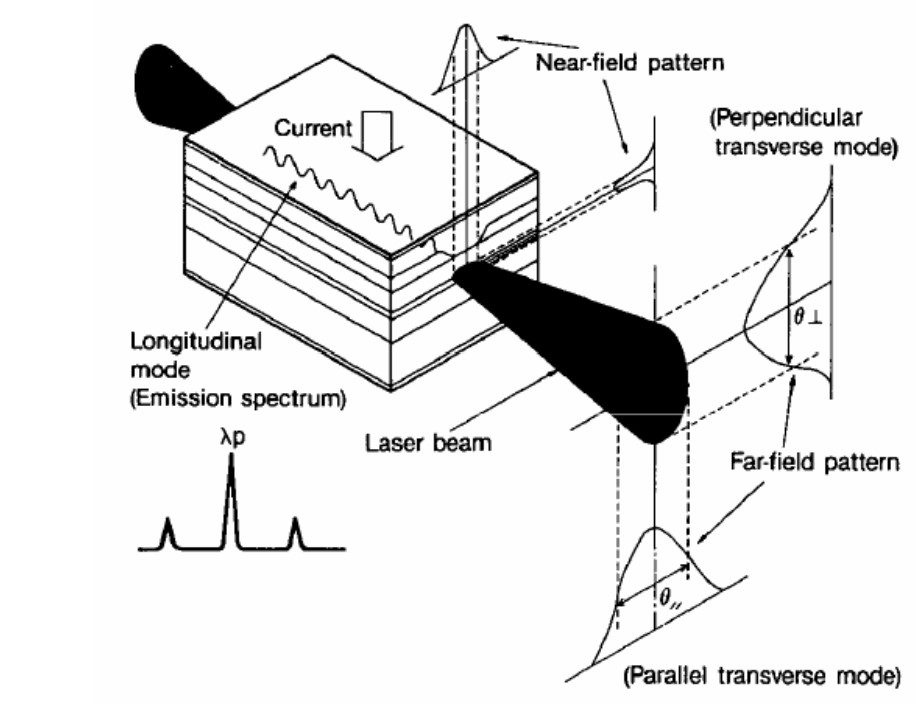
\includegraphics[width=0.5\textwidth]{content/graphics/laserdiodechip.jpg}
    \caption{Schematic view of a laser diode chip.} %\cite
    \label{fig:diodechip}
\end{figure}

The chip consists of a p-doped and a n-doped layer. The p-n junction between the layers is the active Medium.
An excitation current can be connected to the upper and lower ends of the diode to create electron-hole pairs which recombine in the active layer and
emitting light in the process. The current serves as a pump source for the population inversion which occurs in the laser medium.
The wavelength of the emitted light ist approximateley that of the band gab of the semiconductor material.
To create a cavity the claved facets of the chip act as a partically refelceting miorrors.
On this side the light comes out.
Standing waves are formed inside the cavity. The leaving light beam is elliptical and strongly divergent due to the  rectangular shape of the
exit apperature.

The light beam has two unwanted properties which are to be adjusted by an external resonator.
On one hand the light beam has a large linewidth therefore it is unuseable to examine atomic structures.
On the other hand the frequency stability ist very sebsitive to scattering of the emitted light back into the diode.
A Littrow configuration is used in this experiment which is shown in figure \ref{fig:configuration}. 

\begin{figure}[H]
    \centering
    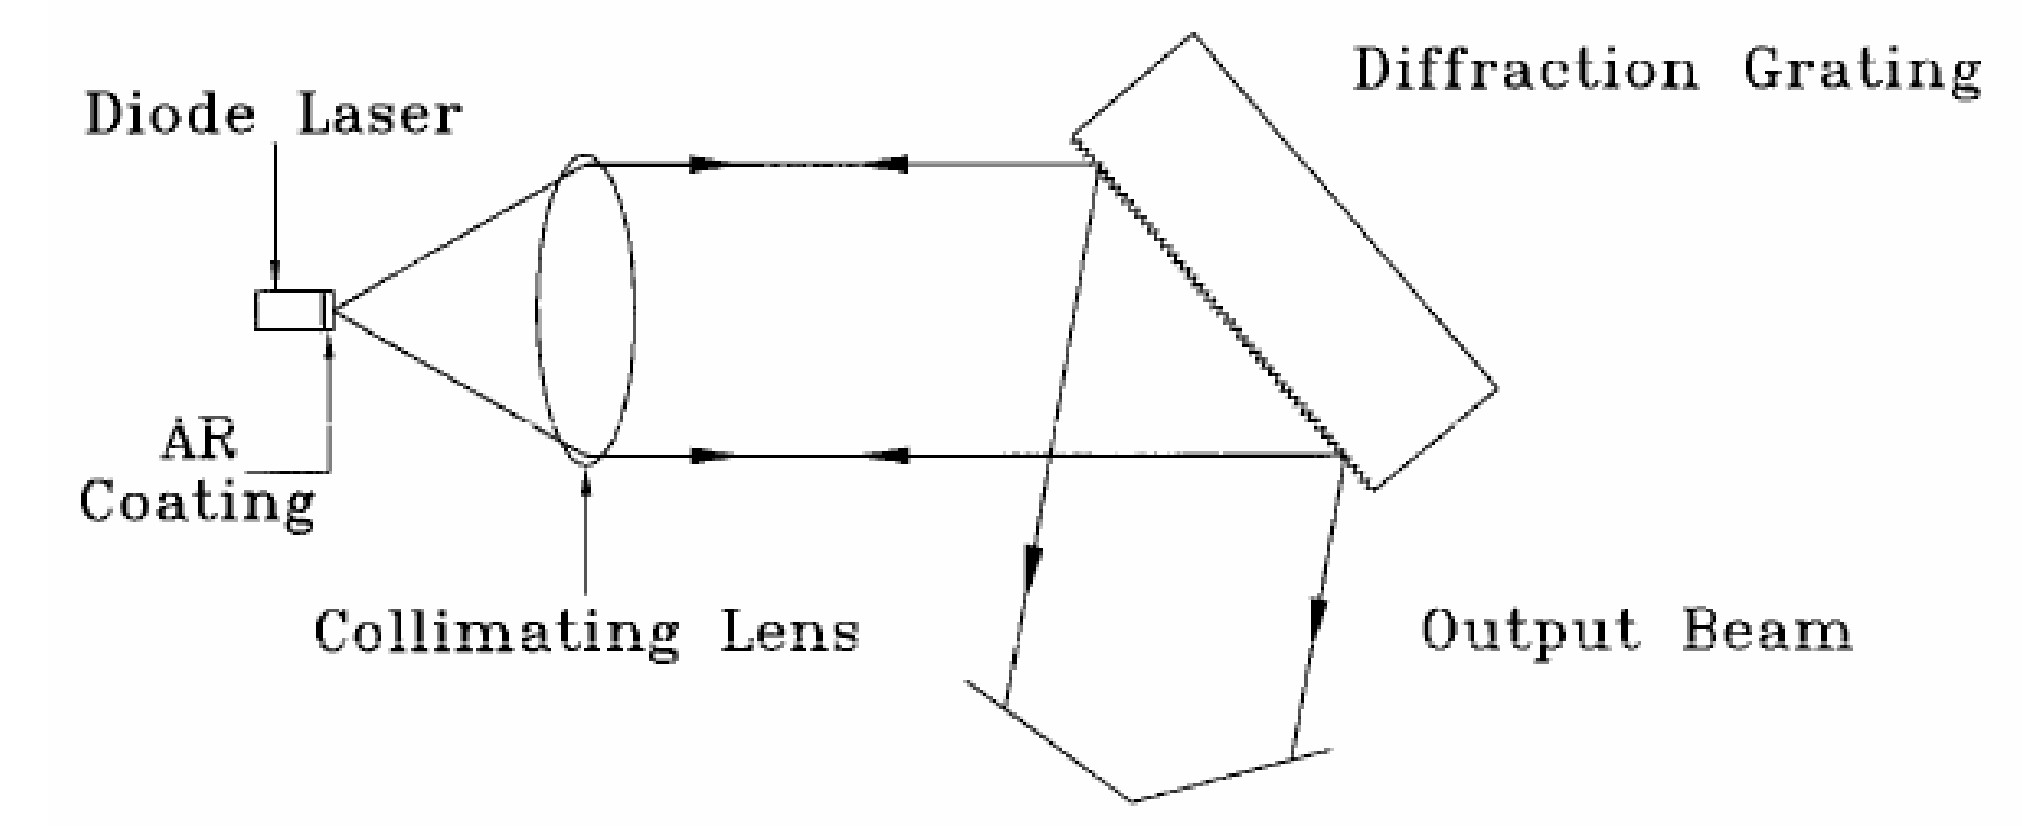
\includegraphics[width=0.8\textwidth]{content/graphics/configuration.jpg}
    \caption{Schematic configuration of the diode laser system.} %\cite
    \label{fig:configuration}
\end{figure}

The external cavity is realized with a lens and a diffraction grating.After leaving the inner cavity the light beam hits a lens which collimate the beam.
Afterwards the light beam encounters the diffration grating. Most of the light directly reflected by the garting  $\left(m = 0 \, \text{grating order}\right)$.
About $ 15 \% $ reflects back into the laser $\left(m = 1  \,\text{grating order}\right)$. The grating forms the external cavity.
This results in a small loss of power, but a much more stable laser beam and a reduced linewidth on $\Delta \nu \approx \qty{1}{\mega\hertz}$.

\subsubsection{Laser Tuning}
\label{sec:Laser Tuning}

To set up the wavelenght of the light emitted by the laser various components must be considered.
Therefore the laser output depends for example on modulation of the current, the temperature of the diode and the postion of the grating.
To understand each component it is important to understand that the laser will tend to lase at the mode frequency with the greatest net gain.
As soon as the laser starts lasing in this mode it results a laser with a single-mode output beam. Under real conditions the laser will sometimes lase 
in two or more modes at the same time. This experiment will concentrate to find a place in parameter space where the laser operates in a single mode.

In Figure \ref{fig:netgain} the wavelength is plotted as a function of the individual amplification modes.The curves are diplaced relative
to one another.

\begin{figure}[H]
    \centering
    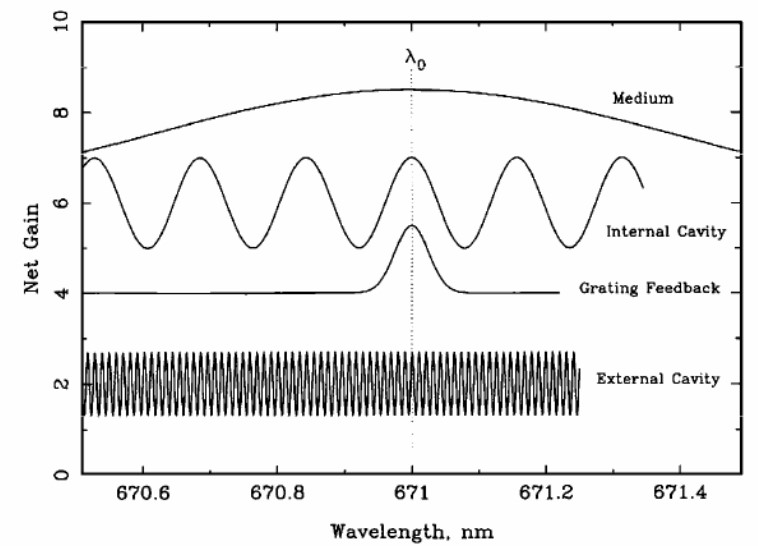
\includegraphics[width=0.5\textwidth]{content/graphics/net_gain_components.jpg}
    \caption{Schematic of the differen constributions to the net gain.} %\cite
    \label{fig:netgain}
\end{figure}

The active medium has a bandgab which depends on the material of the medium. This results a broad peak in the wavelenght distrinution of the amplification.
The peak depends on the temprature of the material. In the case of rubidium for the resonance the temperature should be set so that the laser operates near 
\qty{780}{\nano\meter}.
Dependence is shown in figure \ref{fig:temp}.

\begin{figure}[H]
    \centering
    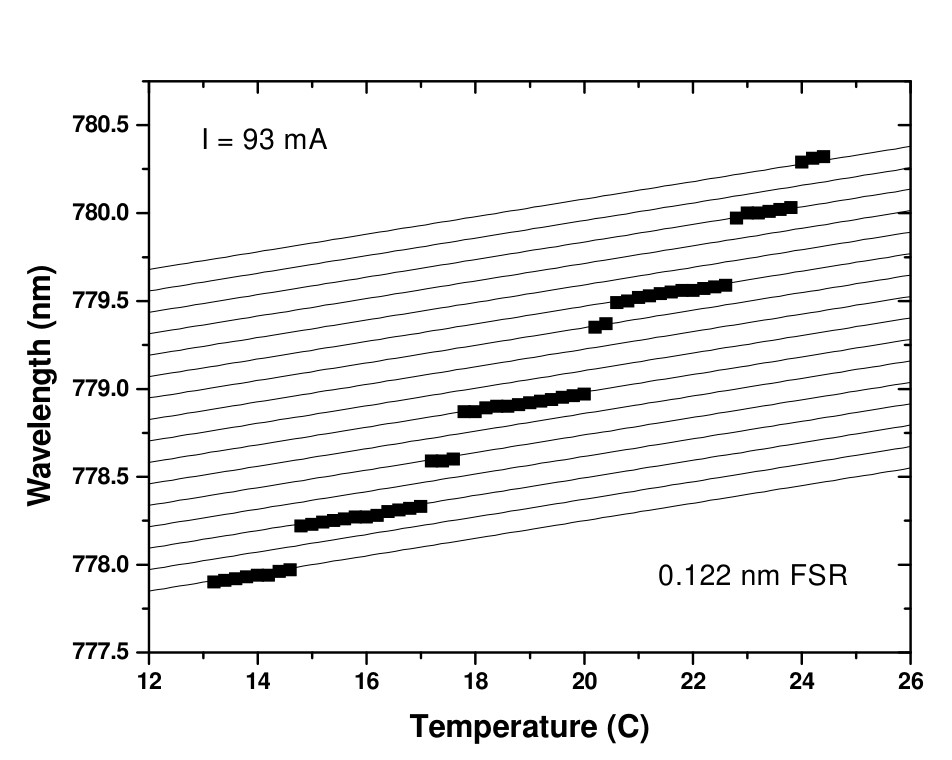
\includegraphics[width=0.5\textwidth]{content/graphics/wavelenghttotemperature.jpg}
    \caption{Dependence of the wavelength on the temperature of the diode.} %\cite
    \label{fig:temp}
\end{figure}

It can be seen that the wavelength correlates with the temperature of the diode.
That means the rising temperature impacts the Bandgab, which shrinks.
Once the medium gain curve is adjusted the cirve is so broad that it is unimportant for net gain.

The internal cavity forms a small Fabry-Perot etalon thus a optical cavity with a normal mode structure. As shown in figure \ref{fig:netgain} the gain function
is periodic in frequency, whereby the period is called free spectral range. Which is given by
\begin{equation}
    \Delta \nu = \frac{c}{2Ln}.
\end{equation}
In this equation $c$ is the speed of light, $n$ is the index of refraction and $L$ is the cavity length.
For the internal cavity the wavelenght of the light depends on the current which is represented in figure \ref{fig:cur}.
The current affects the diode in two ways. First, the diode is heated by the applied current. Second, the current changes the carrier concentration
in the active medium.
\begin{figure}[H]
    \centering
    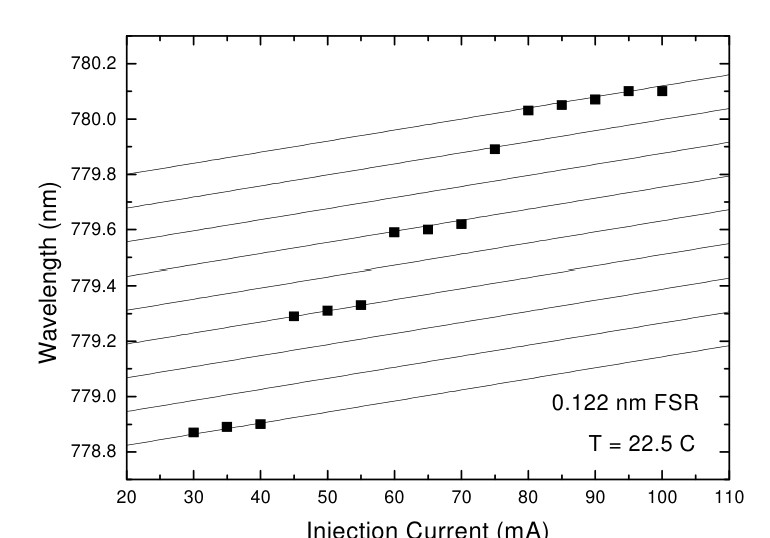
\includegraphics[width=0.5\textwidth]{content/graphics/current.jpg}
    \caption{Dependence of the wavelength on the injection current at a fixed temperature.} %\cite
    \label{fig:cur}
\end{figure}

With a external cavity it is possible that the laser can be made to operate at any wavelength within a reasonably broad range.
Since only light from a narrow wavelength band $\left(m = 1  \,\text{grating order}\right)$ will be fed back into the laser for a fixed grating,
which can be found by 
\begin{equation}
    \lambda = 2 d \sin \theta.
\end{equation}
The size $d$ indicates the line spacing of the grating and $\theta$ is the grating angle. The external cavity ist limited on the one side by the grating and on the
oder side by the refelctive back faced  of the diode. The length of the external cavity is much smaller which results denser peaks in figure \ref{fig:netgain}.
